%%=============================================================================
%% Methodologie
%%=============================================================================


\chapter{\IfLanguageName{dutch}{Methodologie}{Methodology}}%
\label{ch:methodologie}

%% TODO: In dit hoofstuk geef je een korte toelichting over hoe je te werk bent
%% gegaan. Verdeel je onderzoek in grote fasen, en licht in elke fase toe wat
%% de doelstelling was, welke deliverables daar uit gekomen zijn, en welke
%% onderzoeksmethoden je daarbij toegepast hebt. Verantwoord waarom je
%% op deze manier te werk gegaan bent.
%% 
%% Voorbeelden van zulke fasen zijn: literatuurstudie, opstellen van een
%% requirements-analyse, opstellen long-list (bij vergelijkende studie),
%% selectie van geschikte tools (bij vergelijkende studie, "short-list"),
%% opzetten testopstelling/PoC, uitvoeren testen en verzamelen
%% van resultaten, analyse van resultaten, ...
%%
%% !!!!! LET OP !!!!!
%%
%% Het is uitdrukkelijk NIET de bedoeling dat je het grootste deel van de corpus
%% van je bachelorproef in dit hoofstuk verwerkt! Dit hoofdstuk is eerder een
%% kort overzicht van je plan van aanpak.
%%
%% Maak voor elke fase (behalve het literatuuronderzoek) een NIEUW HOOFDSTUK aan
%% en geef het een gepaste titel.

Het doel van dit onderzoek is het identificeren van de meest geschikte pipeline voor de automatisering van het orderproces van een website naar 3D-geprinte producten. Dit proces zal iteratief verlopen, met fasen die zich richten op onderzoek, evaluatie, en prototyping. Elke fase heeft specifieke doelstellingen, deliverables en deadlines. Regelmatige feedback van de Co-promotor zal worden gezocht om de voortgang te evalueren en bij te sturen waar nodig. Ook is het de bedoeling dat deze pipeline zal draaien op Mac en Windows.
\vspace{2em}

\textbf{Fase 1: Literatuurstudie}\\
\textbf{(Deadline: 07 maart 2025)}\\\\
In deze fase wordt er literatuuronderzoek gedaan naar bestaande oplossingen en pipelines die gebruikt kunnen worden voor de automatisering van het orderproces. Dit omvat een analyse van tools zoals Python, integraties met de Shopify API, en printbeheer API's zoals Bambu Studio. De deliverable voor deze fase is een lijst met mogelijke pipelines en tools die geschikt zouden kunnen zijn voor dit project, inclusief voor- en nadelen van elke optie.
\vspace{2em}

\textbf{Fase 2: Proof-of-Concept (PoC)}\\
\textbf{(Deadline: 4 april 2025)}\\\\
Op basis van de literatuurstudie worden meerdere pipelines geselecteerd en getest door een PoC op te zetten voor elke gekozen oplossing. Dit zal helpen om de haalbaarheid van de verschillende pipelines te testen. De PoC zal een order ontvangen via de Shopify API en doorsturen naar de Bambu Studio API. De technische haalbaarheid van elke pipeline wordt geëvalueerd om te bepalen welke het beste presteert.
\vspace{1em}

\textbf{Fase 3: Testen van de Pipelines en Prestatieanalyse}\\
\textbf{(Deadline: 18 April 2025)}\\\\
In deze fase worden de geselecteerde pipelines verder getest. Dit houdt in dat de pipelines onder verschillende belasting- en stressomstandigheden worden getest, zoals het verwerken van meerdere orders tegelijk. Daarnaast wordt er gekeken naar foutafhandelingsmechanismen en de stabiliteit van de integratie met de APIs. Enkele testscenario's omvatten: 
\begin{itemize}
    \item Wat gebeurt er als een bestand mislukt bij het verzenden?
    \item Wat gebeurt er als de printer zonder stroom valt?
    \item Wat gebeurt er bij een printfout?
    \item Hoe wordt het beëindigen van het printproces afgehandeld? 
\end{itemize}
\vspace{1em}

\textbf{Fase 4: Keuze van de Beste Pipeline en Optimalisatie}\\
\textbf{(Deadline: 25 april 2025)}\\\\
Na de uitvoerige tests wordt de beste pipeline geselecteerd op basis van prestaties, fouttolerantie en integratiegemak. In deze fase worden eventuele optimalisaties doorgevoerd en wordt de gekozen oplossing verder verfijnd voor de uiteindelijke implementatie.

\vspace{1em}
\textbf{Dit is de verwachte lijst van Tools:}\\
\begin{itemize}
    \item Python: voor het bouwen van de pipeline en het uitvoeren van API-aanroepen.
    \item Shopify API en Bambu Studio API: om orders te ontvangen en printopdrachten door te sturen.
    \item GitHub: voor versiebeheer van de code en documentatie.
    \item Postman: voor het testen van API-aanroepen tijdens de ontwikkeling.
    \item 3D-printer Bambu Lab X1C: voor het fysiek testen van het printproces.
    \item Verschillende pipelinetools: voor het opzetten en automatiseren van de integratie tussen de verschillende onderdelen van het systeem.
\end{itemize}

\vspace{1em}
\textbf{Dit is de verwachte lijst van functionele vereisten voor de applicatie:}\\
\begin{itemize}
    \item \textbf{MUST}
    \begin{itemize}
        \item Order moet kunnen opgehaald worden  via de API.
        \item Juiste file moet kunnen opgehaald worden.
        \item Printopdracht moet kunnen gestart worden via de API.
    \end{itemize}
    \item \textbf{SHOULD}
    \begin{itemize}
        \item Communicatie naar eigenaar dat print gelsaagd is.
    \end{itemize}
    \item \textbf{COULD}
    \begin{itemize}
        \item Als meerdere orders binnenkomen deze samen plaatsen op het printbed indien mogelijk.
    \end{itemize}
\end{itemize}

\vspace{1em}
\textbf{Planning en deliverables}

\begin{itemize}
    \item Gemaakte flowchart
    
    \begin{figure}[H]  % Use [H] to prevent floating
        \centering
        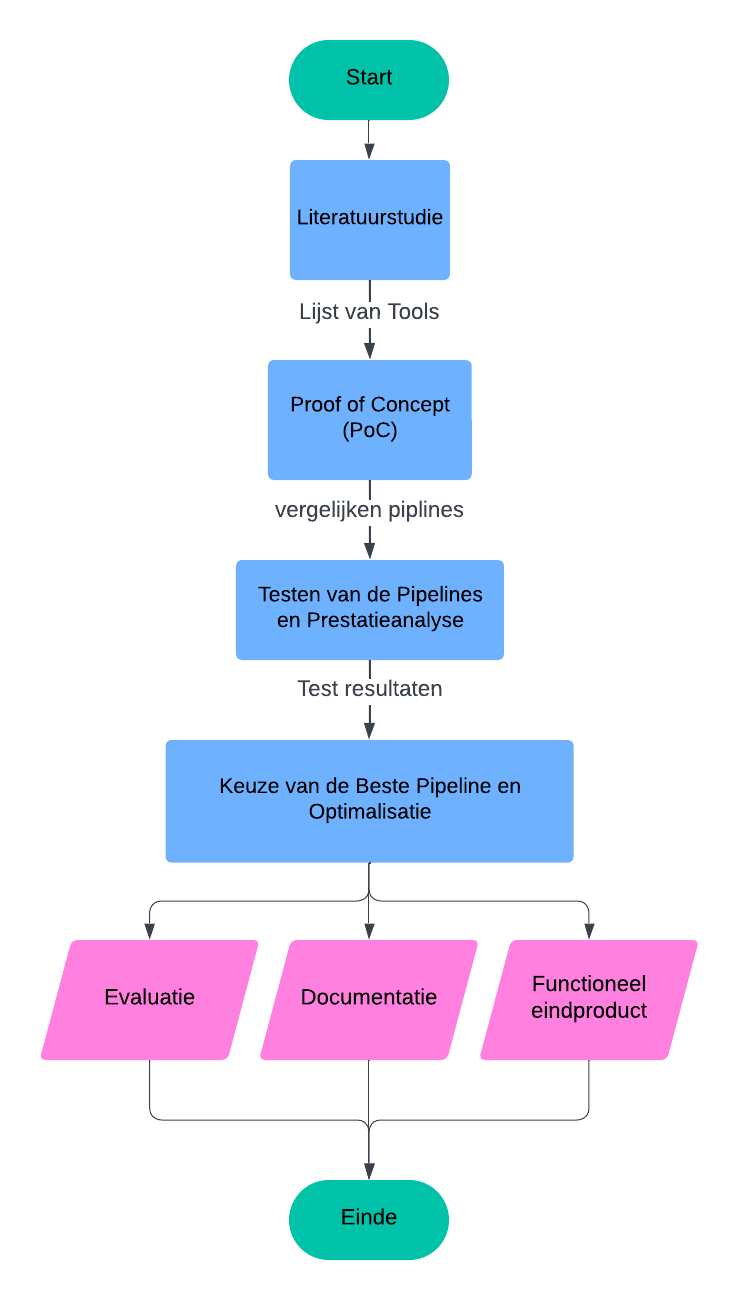
\includegraphics[width=0.5\textwidth]{Flowchart.png}  % Adjust width if necessary
        \caption{Flowchart van verschillende fasen en deliverables van de bachelorproef.}
        \label{fig:flowchart}  % Label for referencing
    \end{figure}
    
    \item Gemaakte Gantt chart.
    
    % Second figure: The Gantt Chart
    \begin{figure}[H]  % Use [H] to prevent floating
        \centering
        \resizebox{\textwidth}{!}{%
            \begin{ganttchart}[
                vgrid,
                hgrid,
                x unit=0.1cm,
                time slot format=isodate,
                compress calendar
                ]{2025-02-01}{2025-05-30}
                
                \gantttitlecalendar{year, month=name} \\
                
                % Fase 1: Literatuurstudie
                \ganttbar[
                progress=100,
                name=litstudie
                ]{Fase 1: Literatuurstudie}{2025-02-01}{2025-02-20} \\
                
                % Fase 2: Proof of Concept (PoC)
                \ganttbar[
                progress=0,
                name=poc
                ]{Fase 2: Proof-of-Concept}{2025-02-21}{2025-04-04} \\
                
                % Fase 3: Experimenten en Testen
                \ganttbar[
                progress=0,
                name=testen
                ]{Fase 3: Testen van de Pipelines en Prestatieanalyse}{2025-04-05}{2025-04-18} \\
                
                % Fase 4: Iteratieve Ontwikkeling en Optimalisatie
                \ganttbar[
                progress=0,
                name=optimalisatie
                ]{Fase 4: Keuze van de Beste Pipeline en Optimalisatie}{2025-04-19}{2025-04-25} \\
                
            \end{ganttchart}
        }
        \caption{Project Planning Gantt Chart}
        \label{fig:ganttchart}  % Label for referencing
    \end{figure}
\end{itemize}


